\usetikzlibrary{decorations.markings,arrows.meta,bending, patterns, math}

\subsection*{Page 183, Problem 11 (ab) (Worked with David LaRoche)}
\vspace{15pt}
\begin{proof}
    \vspace{-10pt}
    \begin{enumerate}[label = (\alph*)]
        \item Join together three copies of the boundary of a triangle at a single vertex as shown below:
        \begin{center} \;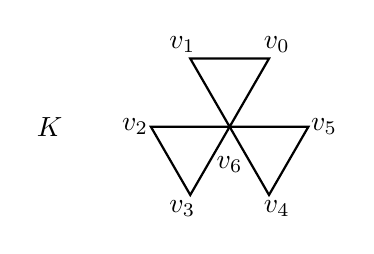
\begin{tikzpicture}
                \tikzset{->-/.style={decoration={
                markings,
                mark=at position #1 with {\arrow{<}}},postaction={decorate}}, ->>-/.style={decoration={
                markings,
                mark=at position #1 with {\arrow{>>}}},postaction={decorate}}}
                
                \node[left = 2cm] (0,0) {$K$};
                \node[below = .25cm] (0,0) {$v_6$};
                \foreach \t/\x in {0/0, 120/2, 240/4}{
                    \tikzmath{\a = \x; \b = int(\x + 1);}
                    \draw[white] (0,0) -- (\t+60:1.2) node[black] {$v_\a$} -- (\t+120:1.2) node[black] {$v_\b$} -- cycle;
                    \draw[thick] (0,0) -- (\t+60:1) -- (\t+120:1) -- cycle;}
        \end{tikzpicture} \end{center}
        $|K|$ is connected so $$H_0(K) = \Z^1 \quad \text{[Theorem 8.2]}.$$ $K$ has fundamental group of a 3-bouquet $F_3$ generated by $z_1 = (v_6v_1) + (v_1v_0) + (v_0v_6)$, $z_2 = (v_6v_5) + (v_5v_4) + (v_4v_6)$, and $z_3 = (v_6v_3) + (v_3v_2) + (v_2v_6).$ Thus, its abelianization \[\langle z_1, z_2, z_3 \mid z_1z_2z_1^{-1}z_2^{-1}, z_1z_3z_1^{-1}z_3^{-1}, z_2z_3z_2^{-1}z_3^{-1} = e \rangle\] is equal to $$H_1(K) \cong \Z^3\quad \text{[Theorem 8.3]}.$$ There are no 2 - or higher - simplexes so $B_{\geq 2}(K), Z_{\geq 2}(K) = \{0\}$ and $$H_q(K) = \{0\} \quad q \geq 2.$$

        \item We can glue two hollow tetrahedra along an edge to get the following:
        \begin{center}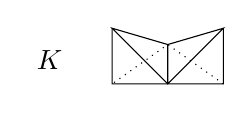
\begin{tikzpicture}
            \tikzset{->-/.style={decoration={
            markings,
            mark=at position #1 with {\arrow{<}}},postaction={decorate}}, ->>-/.style={decoration={
            markings,
            mark=at position #1 with {\arrow{>>}}},postaction={decorate}}}
            
            \node[xshift = -1.5cm, yshift = .3cm] (0,0) {$K$};
            \draw (0,0) -- (45:1) -- (90:.5) -- (135:1) -- cycle -- (90:.5);
            \draw (0,0) -- (0:.707) -- (45:1);
            \draw (0,0) -- (180:.707) -- (135:1);
            \draw[dotted] (0:.707) -- (90:.5) -- (180:.707);
        \end{tikzpicture} \end{center}
        $|K|$ is connected so $$H_0(K) = \Z^1 \quad \text{[Theorem 8.2]}.$$ Note that each empty tetrahedra is homeomorphic to $S^2$ so they have the same homotopy type. Because they're path-connected, they have isomorphic fundamental groups $\{e\}$. Now, by Van Kampen's theorem, $K$ has the same fundamental group as the one point union of 2-spheres and thus has fundamental group equal to the free product of each trivial group which is itself the trivial group. Thus, $\pi_1(K)$'s abelianization gives $$H_1(K) = \{0\}\quad \text{[Theorem 8.3]}.$$ There are no complexes of dimension 3 or greater so $B_2(K)$, $B_3(K)$, $\cdots = \{0\}$ and $Z_3(K), Z_4(K), \cdots = \{0\}$. We can therefore show $H_2(K) = Z_2(K)/\{0\} = \text{Ker } \partial\colon C_{2}(K)\to C_{1}(K) \cong \Z^2$ as follows. Pick any 2-simplex to start. To annihilate the boundary of any 2-chain starting at this triangle, we MUST orient it compatibly with another 2-simplex on the same tetrahedron in order to kill their shared edge. This requires another 2-simplex on the same tetrahedron by the same argument and then the last one, all on one tetrahedron. This has already killed the boundary so its clear any 2-cycle can be decomposed into scalar multiples of these isolated 2-cycles on each tetrahedredon. Therefore, they together generate $Z(K)$. Addition of these cycles is commutative so the abelianization gives $\Z(K) \cong \Z^2$. Thus, $$H_2(K) = Z_2(K)/\{0\} \cong \Z^2.$$ Given what we said about $Z_3(K), Z_4(K), \cdots$ and $B_3(K), B_4(K), \cdots$, $$H_q(K) = \{0\} \quad q \geq 3.$$
    \end{enumerate}
\end{proof}

\subsection*{Page 183, Problem 13}
\vspace{15pt}
\begin{proof}
    \vspace{-10pt}
    Take any (path-connected) graph $\Gamma$ with maximal tree $T$. $G(\Gamma,T)$ by construction includes only the generators $g_{ij}$ ($i <j$) of edges of $\Gamma-T$ each `representing' exactly one non-2-simplex triangle (a triangle made of 3 1-simplices which is not filled in). Recall every such triangle also has only this generator. $T$ is clearly contractible and can be thought of as a single vertex from which each edge generator is independently attached so that $G(\Gamma, T)$ is isomorphic to the free group on $n$ generators where $n$ is the number of such edges. (Recall specifically there are no relations in $G(\Gamma, T)$ as $T$ is maximal and an edge path contained entirely within $T$ can always be found from the basepoint to some generator and back implying the generators are indpendent.) Last, $\Gamma$ is path-connected so $G(\Gamma,T)$ is isomorphic to $\pi_1(\Gamma, v)$ regardless of choice of $v$. 
    
    This same result can also be achieved through repeatedly applying Van Kampen's theorem on $T$ and one empty triangle at a time which would each time give just the generating loop of that triangle with the single relation that that loop 0 times is the identity, i.e. the trivial relation and therefore a free group on $\beta_1$ generators.

    The homeomorphic reduction of 2-simplices first into one of their respective line-segment components and then all of $T$'s `spikes' down into just one point leaving only empty triangles implies $\Gamma$ shares the exact homotopy type as a bouquet of circles. This also implies their isomorphic fundamental groups.
        
    Now by Theorem 8.3, the abelianization of $F_n$ gives $\overbrace{\Z \oplus \cdots \oplus \Z}^{n \text{ times}} \cong \Z^n$ as the first homology group of $\Gamma$. $H_1(\Gamma)$ has no torsion element so the first Betti number of $\Gamma$ is the rank of $\Z^n$, i.e. n, i.e. the number of not-filled-in triangles in the graph = $\beta_1$. 

\end{proof}

\subsection*{Page 188, Problem 20}
\vspace{15pt}
\begin{proof}
    \vspace{-10pt}
    Take chain maps $\phi\colon C(K)\to C(L)$, $\psi\colon C(L)\to C(M)$. Because $\partial\circ\phi_q = \phi_{q-1}\circ\partial$ and $\partial\circ\psi_q = \psi_{q-1}\circ\partial$, we know that $$\partial\circ(\psi_q\circ\phi_q) = (\partial\circ\psi_q)\circ\phi_q=(\psi_{q-1}\circ\partial)\circ\phi_{q}=(\psi_{q-1}\circ\phi_{q-1})\circ\partial.$$
    (Generically, we can show our induced map is well-defined via the following. For normal subgroups $N \vartriangleleft G, M \vartriangleleft H$ and $f\colon G\to H$, if $f(N) \subseteq M$ then $f_*\colon G/N \to H/M$ is well-defined as for any cosets $g_1 + N = g_2 + N$, $f(g_1) + M = f(g_1) + f(N) + M = f(g_1 + N) + M = f_*(g_1 + N) = f_*(g_2+N) = f(g_2 + N) + M = f(g_2) + f(N) + f(M) = f(g_2) + M$. This is trivially a homomorphism too.)

    Thus, to show $\psi\circ\phi$ induces a homomorphism $(\psi\circ\phi)_{*}\colon H_q(K)\to H_q(M)$, we need only show $\psi_q\circ\phi_q(Z_q(K)) \subseteq Z_q(M)$ and $\psi_q\circ\phi_q(B_q(K)) \subseteq B_q(M)$. This is implied (via the proof on page 185) by the fact that both $\psi, \phi$ are chain maps and therefore \begin{align*}\psi_q\circ\phi_q(Z_q(K))\subseteq \psi_q(Z_q(L))\subseteq Z_q(M),\\ \psi_q\circ\phi_q(B_q(K))\subseteq \psi_q(B_q(L))\subseteq B_q(M).\end{align*} Thus, $\psi\circ\phi$ is a chain map and by the above containments, for any $z \in Z_q(K)$, we get $(\psi\circ\phi)_*(z+B_q(K)) = (\psi\circ\phi)(z + B_q(K)) + B_q(M) = (\psi\circ\phi)(z) + \psi\circ\phi(B_q(K)) + B_q(M) = (\psi\circ\phi)(z) + B_q(M) = (\psi\circ\phi)(z) + \psi(B_q(L)) + B_q(M) = \psi(\phi(z) + B_q(L)) + B_q(M) = \psi_*(\phi(z) + B_q(L)) = \psi_*(\phi(z) + \phi(B_q(K)) + B_q(L)) = \psi_*(\phi(z + B_q(K)) + B_q(L)) = \psi_*(\phi_*(z+B_q(K))) = \psi_*\circ\phi_*(z+B_q(K))$. $z$ is arbitrary so $(\psi\circ\phi)_* = \psi_*\circ\phi_*$.
\end{proof}

\subsection*{Page 192, Problem 25}
\vspace{15pt}
\begin{proof}
    \vspace{-10pt}
    Take similicial maps $s,t\colon|K|\to|L|$. Suppose there exists a homomorphism $d_q\colon C_q(K)\to C_{q+1}(L)$ for all $q$ so that $$d_{q-1}\partial + \partial d_q = t-s\colon C_q(K)\to C_{q+1}(L).$$ Then for any $z \in Z_q(K)$, $\partial(z) = 0$ and $d_q(z) \in C_{q+1}(L) \implies \partial d_q(z) \in B_q(L)$. This means $t(z) - s(z) = d_{q-1}\partial(z) + \partial(d_q(z)) = 0 + \partial d_q(z) \in B_q(L)$ and consequently that $t_*(z) - s_*(z) = [0]$ so finally $t_*(z) = s_*(z)$ for all $z$. Thefore $s,t$ induce the same homomorphism $s_* = t_*\colon H_q(K) \to H_q(L)$.
\end{proof}